\documentclass[]{elsarticle} %review=doublespace preprint=single 5p=2 column
%%% Begin My package additions %%%%%%%%%%%%%%%%%%%
\usepackage[hyphens]{url}

  \journal{Journal of Transport \& Health} % Sets Journal name


\usepackage{lineno} % add
\providecommand{\tightlist}{%
  \setlength{\itemsep}{0pt}\setlength{\parskip}{0pt}}

\usepackage{graphicx}
%%%%%%%%%%%%%%%% end my additions to header

\usepackage[T1]{fontenc}
\usepackage{lmodern}
\usepackage{amssymb,amsmath}
\usepackage{ifxetex,ifluatex}
\usepackage{fixltx2e} % provides \textsubscript
% use upquote if available, for straight quotes in verbatim environments
\IfFileExists{upquote.sty}{\usepackage{upquote}}{}
\ifnum 0\ifxetex 1\fi\ifluatex 1\fi=0 % if pdftex
  \usepackage[utf8]{inputenc}
\else % if luatex or xelatex
  \usepackage{fontspec}
  \ifxetex
    \usepackage{xltxtra,xunicode}
  \fi
  \defaultfontfeatures{Mapping=tex-text,Scale=MatchLowercase}
  \newcommand{\euro}{€}
\fi
% use microtype if available
\IfFileExists{microtype.sty}{\usepackage{microtype}}{}
\bibliographystyle{elsarticle-harv}
\usepackage{graphicx}
\ifxetex
  \usepackage[setpagesize=false, % page size defined by xetex
              unicode=false, % unicode breaks when used with xetex
              xetex]{hyperref}
\else
  \usepackage[unicode=true]{hyperref}
\fi
\hypersetup{breaklinks=true,
            bookmarks=true,
            pdfauthor={},
            pdftitle={How do school travel planning stakeholders frame active school travel in Ontario, Canada?},
            colorlinks=false,
            urlcolor=blue,
            linkcolor=magenta,
            pdfborder={0 0 0}}
\urlstyle{same}  % don't use monospace font for urls

\setcounter{secnumdepth}{0}
% Pandoc toggle for numbering sections (defaults to be off)
\setcounter{secnumdepth}{0}

% Pandoc citation processing

% Pandoc header
\usepackage{booktabs}
\usepackage{longtable}
\usepackage{array}
\usepackage{multirow}
\usepackage{wrapfig}
\usepackage{float}
\usepackage{colortbl}
\usepackage{pdflscape}
\usepackage{tabu}
\usepackage{threeparttable}
\usepackage{threeparttablex}
\usepackage[normalem]{ulem}
\usepackage{makecell}
\usepackage{xcolor}



\begin{document}
\begin{frontmatter}

  \title{How do school travel planning stakeholders frame active school travel in
Ontario, Canada?}
    \author[Some Department]{Author 1\corref{1}}
   \ead{author1@example.com} 
    \author[Some Department]{Author 2}
   \ead{author2@example.com} 
    \author[Another University]{Author 3\corref{2}}
   \ead{author3@example.com} 
    \author[Some Institute]{Author 4\corref{2}}
   \ead{author4@example.com} 
    \author[Some University]{Author 5}
   \ead{author5@example.com} 
    \author[Some Department]{Author 6}
   \ead{author6@example.com} 
      \address[Some Department]{Department, Street, City, Province, Postal Code}
    \address[Another University]{Department, Street, City, Province, Postal Code}
    \address[Some Institute]{Street, City, Province, Postal Code}
    \address[Some University]{Department, Street, City, Province, Postal Code}
      \cortext[1]{Corresponding Author}
    \cortext[2]{Equal contribution}
  
  \begin{abstract}
  This is the abstract.
  
  It consists of two paragraphs.
  \end{abstract}
  
 \end{frontmatter}

\textbf{\emph{Background}}:\\
\textbf{\emph{Methods}}:\\
\textbf{\emph{Results}}: \textbf{\emph{Conclusions}}:

\newpage

\hypertarget{introduction}{%
\section{1. Introduction}\label{introduction}}

Walking and bicycling to school, commonly known as active school travel
(AST), has been declining in Canada and North America for decades
({\textbf{???}}), with levels much lower than other developed countries
like The Netherlands ({\textbf{???}}) and Japan ({\textbf{???}}). In
response to this trend, school travel planning has become a popular
intervention across Canada that has resulted in mixed success with some
schools reporting an increase in AST (e.g., {\textbf{???}}; Mammen et
al., 2014), while others did not observe a change in behaviour
(Buttazzoni et al., 2019) or needed more time and resources to be
effective ({\textbf{???}}).

School travel planning (STP) is a ``school-specific'' intervention led
by a facilitator that brings together a committee of stakeholders from
diverse sectors including education, planning, transportation, and
public health to develop action plans ({\textbf{???}}). This five-step
process involves identifying barriers to AST based on the local context
and implementing approaches or activities that alleviate concerns and
encourage AST ({\textbf{???}}). STP facilitators and committee members
generally intervene at the school through a range of activities such as
educational strategies, in-person events or programs, improvements to
the school site, and enforcement (Mammen et al., 2014).

How STP is framed to a target audience may influence how this
intervention is received and whether it encourages the audience to
support it or participate. In particular, STP stakeholders make choices
about the points of intervention and potential benefits that ought to be
communicated to the public to facilitate adoption of AST. Educational
strategies, which account for approximately one quarter of STP
strategies implemented at Canadian schools (Mammen et al., 2014), need
to effectively engage multiple audiences -- parents, students,
politicians -- on the issue, challenges, and benefits of AST.
Promotional materials, therefore, should reflect current knowledge from
research about school travel and the built environment, as well as local
content specific to factors that influence travel decisions for parents,
in order to effectively engage the public in advocating for improving
AST or to expose parents and the community to essential information that
may prompt behaviour change.

On the one hand, parents have been found to express different
understandings, nomenclature, and conceptualizations than planners of
the factors that influence school travel (Buliung et al., 2021).
However, it is unknown to what degree there is concurrence between STP
materials presented to the public and the literature on school travel
and parental perceptions, and how the complexity of the AST issue is
presented to the public.

The aim of this paper is to fill this research gap by analyzing how AST
is framed by STP stakeholders in Ontario, Canada. We used text mining
and topic modelling to examine how local policy documents from Ontario
municipalities and school boards present and communicate the benefits
and barriers of AST and the solutions for improving AST. We compared the
findings from these documents to a selection of studies on AST and
explored the extent to which there is concurrence between research
findings to date and promotional materials shared with the public to
increase AST.

\hypertarget{literature-review}{%
\section{2. Literature Review}\label{literature-review}}

\hypertarget{data}{%
\section{3. Data}\label{data}}

\hypertarget{data-retrieval}{%
\subsection{3.1. Data retrieval}\label{data-retrieval}}

\hypertarget{policy-documents}{%
\subsubsection{3.1.1. Policy documents}\label{policy-documents}}

We assembled a collection of publicly available documents that were
sourced online from the main stakeholder groups involved in STP
initiatives in Ontario: i) school boards (public and English-speaking
only); ii) municipal governments; and iii) transportation consortia.
Non-profit organizations, police services, and advocacy groups are other
stakeholders who may play a role in supporting AST and/or STP, but this
study does not include any documents from these groups because they are
not consistently participating in all initiatives.

The search was guided first by a list of all English public school
boards across Ontario. The websites of each school board were manually
searched for pages related to school transportation or travel. Any pages
relevant to these topics were manually downloaded. Next, we collected
documents by searching municipal government and transportation consortia
websites. The latter were identified based on geographic area (i.e., the
municipalities and/or transportation consortia that are in the same
geographic area of each school board). Pages related to active or school
travel were manually downloaded. Webpages from STP stakeholder websites
were included in our analysis if they were easy to find. This primary
criteria was important since our analysis pertains to how such issues
are framed to the public. Thus, we included only webpages that were easy
to find, which we defined as requiring no more than 2-4 separate links
from the initial Google search.

The initial corpus of policy documents included 64 relevant webpages
(i.e., one page or more) from all STP stakeholder groups. It is
important to note that school boards, municipalities, and transportation
consortia may or may not publish information about their involvement in
AST and STP efforts on their respective websites or in policy documents,
which means that some of these groups for particular regions in Ontario
are not included in our analysis. Search results are summarized in Table
\ref{tab:policy-documents}.

\begin{table}

\caption{\label{tab:policy-documents}\label{tab:search-results}Search results from the main STP stakeholder groups.}
\centering
\resizebox{\linewidth}{!}{
\begin{tabular}[t]{>{}l|l|>{}l}
\toprule
Stakeholder & Total & Included\\
\midrule
\cellcolor{gray!6}{\textbf{School boards}} & \cellcolor{gray!6}{62} & \cellcolor{gray!6}{31}\\
\textbf{Municipalities} & 62 & 25\\
\cellcolor{gray!6}{\textbf{Transportation consortia}} & \cellcolor{gray!6}{39} & \cellcolor{gray!6}{8}\\
\bottomrule
\end{tabular}}
\end{table}

\hypertarget{academic-papers}{%
\subsubsection{3.2.1. Academic papers}\label{academic-papers}}

\textbf{To be completed by Dr.~Paez}

\hypertarget{data-cleaning}{%
\subsection{3.2. Data cleaning}\label{data-cleaning}}

A multi-step process was conducted to ensure that the analysis captured
as much content as possible from both the policy documents (n = 64) and
academic papers (n = 233). To begin, the webpages, which were manually
downloaded in portable document format (PDF), were trimmed so that pages
that only consisted of tables, figures, or references were removed. Many
academic papers were in a two-column format, which is not ideal for
conversion to \texttt{txt}. We adapted a procedure
(https://stackoverflow.com/questions/42541849/extract-text-from-two-column-pdf-with-r)
to read the two-column PDF documents so that they would be converted
correctly. Four academic papers did not join sufficiently and were taken
out of the corpus due to the substantial time required to manually
correct their inconsistencies.

Next, we converted the trimmed PDF documents into \texttt{txt} files so
that they could be imported in R for analysis. We then proceeded to a
manual cleaning phase where we removed any remaining tables, figures,
references, headers/footings, and captions that could not be trimmed.
Manual corrections were also required for certain pages in academic
papers that remained in two-column format after the conversion process.
This typically occurred on pages that had a table or figure which
disrupted the text. Finally, we reviewed all of the documents to remove
hyphenation by line breaks and to keep hyphenated words together on the
same line. Any ligatures (e.g., combinations of characters or letters
that were not properly detected during the conversion process) were
fixed by inserting the unicode sequence of character to replace the
missing sequence of characters.

We also manually removed any extraneous material in the academic papers
that did not pertain to AST specifically. This included footnotes,
references, acknowledgments, and conflict of interest statements in the
academic papers. We removed all phone numbers, inserted links to other
webpages, personal names, and content not to specific to AST from the
policy documents that were retrieved from the websites of school boards,
municipalities, and transportation consortia.

In the final step, we removed all blank spaces, punctuation,
capitalization, and numbers. English stop words, which are common words
such as \emph{and} or \emph{the} as identified in a predetermined list
by Lewis et al.~({\textbf{???}}) and other frequent terms in the
documents like ``school'' and specific location names, were removed from
the corpora.

\hypertarget{methods}{%
\section{4. Methods}\label{methods}}

\hypertarget{framing-analysis}{%
\subsection{4.1. Framing analysis}\label{framing-analysis}}

Issues that pertain to public health or wellbeing are often presented to
the public through particular frames to influence perceptions or
behaviours. Gamson and Modigliani ({\textbf{???}}) conceptualize a frame
as a ``central organizing idea or story line that provides meaning'' to
a particular phenomenon. A frame can enable individuals ``to locate,
perceive, identify, and label'' information pertaining to various
dimensions of an issue (Goffman, 1974). Scholars in the field of
political communications have proposed that communicators, such as the
media or an institution, construct the narrative of a frame for policy
positions or public issues in order to activate or restrict a particular
response in the intended audience (Pan and Kosicki, 1993). Framing can
be used to position existing solutions as suitable to address particular
issues (Mah et al., 2014), which may prevent the public from being aware
of other policy approaches that challenge the status quo to bring about
more radical change. The way policy issues are framed is ultimately
important to understand because it plays a role in either altering or
preserving the existing social perceptions.

Framing of issues is an important step in developing health policy. An
obvious example over the past decade is the framing of climate change as
a public health issue (e.g., @ depouxCommunicatingClimateChange2017;
Maibach et al., 2010; Weathers and Kendall, 2016) to increase public
engagement and reception of the issue. Transport planners also use
different frames to guide the extent to which transport policies can be
adapted to address climate change. In a recent paper ({\textbf{???}}),
framing analysis was applied to review the representation of issues such
as mobility and social exclusion in municipal policies from four western
Canadian cities under the current circumstances of climate change. The
authors found four primary frames: ``The Growing City'', ``If You Build
It, They Will Come'', ``Better City for All'', and a ``the Resilient
City''. Each frame presented the nature, opportunities, and challenges
of climate change in different ways which set the stage for the types of
mitigation and adaptation strategies that cities were proposing to
address this issue.

Given the range of factors at multiple levels of the socioecological
model that influence school travel, it is important to understand how
walking and bicycling to school are framed to the public. Is active
school travel framed as a public health or environmental issue? Is it
framed as both? Do proposed solutions to increase AST focus primarily on
the intrapersonal and interpersonal factors, meaning that behaviour
change must ultimately result from different decisions made by the
individual or the household? Or is the decline in AST framed as an issue
that must be addressed through changes in the built environment? These
are the types of questions that we aim to answer in this paper. To our
knowledge, this topic has not be addressed in the school travel
literature to date.

\hypertarget{topic-modelling}{%
\subsection{4.2. Topic modelling}\label{topic-modelling}}

The topic modelling analysis was conducted in R. We primarily used the
following packages: \texttt{topicmodels} ({\textbf{???}}),
\texttt{word2vec} ({\textbf{???}}), and \texttt{wordcloud}
({\textbf{???}}) to examine content in the documents that were sourced
for this project. These packages have functions for determining the
frequency of specific words in each document, relationships (e.g., pairs
of adjacent terms) and correlations between words, and estimating Latent
Dirichlet allocation (LDA) models to classify documents according to the
topics that are contained within them. We describe in the section below
how we used these functions to produce our results.

\hypertarget{reproducibility}{%
\subsection{4.3. Reproducibility}\label{reproducibility}}

This paper is an example of open and reproducible research that uses
only open software. All data were obtained from publicly available
sources and organized in the form of a data package. Following best
practices in spatial data science ({\textbf{???}}), the code and data
needed to reproduce or conduct a similar analysis for other regions in
North America or elsewhere are available for download.

\hypertarget{results}{%
\section{5. Results}\label{results}}

\hypertarget{word-and-document-frequency}{%
\subsection{5.1. Word and document
frequency}\label{word-and-document-frequency}}

We analyzed word and document frequency for each corpora. Table
\ref{tab:word-table} shows the most frequent terms found in the
municipal, transportation consortia, school board, and academic
documents. As expected, STP documents and academic papers reference
\emph{active travel}, \emph{walking}, \emph{biking} or \emph{cycling},
and \emph{students} more than other terms. Each corpora also has
\emph{safety} and \emph{traffic} as common words which suggests
congruence on these key factors between the research literature and how
AST is framed to the public. The word \emph{physical} is present in each
corpus which could refer to either \emph{physical activity},
\emph{physical health}, or the \emph{physical environment}. Furthermore,
documents from STP stakeholders discuss \emph{resources},
\emph{information}, and \emph{services} about school travel. In the
section below, the context in which these terms appear is explored
further through their concordance. Unlike the academic papers, STP
stakeholder documents include the words \emph{route} or \emph{routes}.
This could reflect their role in identifying safe routes to school to
share with parents or families, as well as the STP emphasis on making
the physical environment safer for AST. The academic corpora differs
from the policy documents in that \emph{parents} and \emph{distance} are
the second and third most common terms. In addition, \emph{time},
\emph{factors}, \emph{environment}, and \emph{age} are also identified
in academic papers. These words are absent from the list of common words
in policy documents. Table \ref{tab:word-table} indicates that the
research corpora discusses a broader range of determinants of AST than
the policy documents. The number of references for each term in the
academic papers is also significantly higher due to the inclusion of
more documents.

\begin{table}

\caption{\label{tab:word-table}\label{tab:word-table}Top 25 terms identified in each corpora. Document frequencies are also indicated.}
\centering
\resizebox{\linewidth}{!}{
\begin{tabular}[t]{lcclcclcclcc}
\toprule
\multicolumn{3}{c}{Municipalities} & \multicolumn{3}{c}{School Boards} & \multicolumn{3}{c}{Transportation Consortia} & \multicolumn{3}{c}{Academic Papers} \\
\cmidrule(l{3pt}r{3pt}){1-3} \cmidrule(l{3pt}r{3pt}){4-6} \cmidrule(l{3pt}r{3pt}){7-9} \cmidrule(l{3pt}r{3pt}){10-12}
Term & Count (n) & Documents (n) & Term & Count (n) & Documents (n) & Term & Count (n) & Documents (n) & Term & Count (n) & Documents (n)\\
\midrule
\cellcolor{gray!6}{active} & \cellcolor{gray!6}{248} & \cellcolor{gray!6}{26} & \cellcolor{gray!6}{active} & \cellcolor{gray!6}{124} & \cellcolor{gray!6}{13} & \cellcolor{gray!6}{active} & \cellcolor{gray!6}{67} & \cellcolor{gray!6}{7} & \cellcolor{gray!6}{walking} & \cellcolor{gray!6}{5137} & \cellcolor{gray!6}{222}\\
travel & 126 & 20 & bus & 120 & 20 & walking & 55 & 8 & parents & 3946 & 211\\
\cellcolor{gray!6}{walking} & \cellcolor{gray!6}{90} & \cellcolor{gray!6}{25} & \cellcolor{gray!6}{travel} & \cellcolor{gray!6}{103} & \cellcolor{gray!6}{11} & \cellcolor{gray!6}{walk} & \cellcolor{gray!6}{49} & \cellcolor{gray!6}{8} & \cellcolor{gray!6}{distance} & \cellcolor{gray!6}{3271} & \cellcolor{gray!6}{205}\\
bike & 87 & 15 & information & 65 & 21 & travel & 41 & 8 & students & 2960 & 173\\
\cellcolor{gray!6}{cycling} & \cellcolor{gray!6}{78} & \cellcolor{gray!6}{22} & \cellcolor{gray!6}{walking} & \cellcolor{gray!6}{57} & \cellcolor{gray!6}{17} & \cellcolor{gray!6}{students} & \cellcolor{gray!6}{39} & \cellcolor{gray!6}{9} & \cellcolor{gray!6}{cycling} & \cellcolor{gray!6}{2753} & \cellcolor{gray!6}{171}\\
\addlinespace
safety & 71 & 21 & walk & 53 & 13 & safety & 32 & 6 & environment & 2631 & 202\\
\cellcolor{gray!6}{health} & \cellcolor{gray!6}{65} & \cellcolor{gray!6}{21} & \cellcolor{gray!6}{weather} & \cellcolor{gray!6}{40} & \cellcolor{gray!6}{11} & \cellcolor{gray!6}{help} & \cellcolor{gray!6}{29} & \cellcolor{gray!6}{9} & \cellcolor{gray!6}{activity} & \cellcolor{gray!6}{2371} & \cellcolor{gray!6}{209}\\
physical & 63 & 18 & safety & 40 & 19 & schools & 25 & 9 & traffic & 2353 & 208\\
\cellcolor{gray!6}{traffic} & \cellcolor{gray!6}{59} & \cellcolor{gray!6}{20} & \cellcolor{gray!6}{safe} & \cellcolor{gray!6}{39} & \cellcolor{gray!6}{19} & \cellcolor{gray!6}{children} & \cellcolor{gray!6}{25} & \cellcolor{gray!6}{6} & \cellcolor{gray!6}{choice} & \cellcolor{gray!6}{2299} & \cellcolor{gray!6}{169}\\
road & 56 & 13 & services & 37 & 17 & community & 24 & 7 & physical & 2256 & 215\\
\addlinespace
\cellcolor{gray!6}{activity} & \cellcolor{gray!6}{55} & \cellcolor{gray!6}{14} & \cellcolor{gray!6}{planning} & \cellcolor{gray!6}{37} & \cellcolor{gray!6}{7} & \cellcolor{gray!6}{bus} & \cellcolor{gray!6}{18} & \cellcolor{gray!6}{4} & \cellcolor{gray!6}{trips} & \cellcolor{gray!6}{2194} & \cellcolor{gray!6}{170}\\
schools & 52 & 14 & parents & 32 & 17 & route & 17 & 5 & car & 2148 & 195\\
\cellcolor{gray!6}{children} & \cellcolor{gray!6}{47} & \cellcolor{gray!6}{15} & \cellcolor{gray!6}{sustainable} & \cellcolor{gray!6}{31} & \cellcolor{gray!6}{8} & \cellcolor{gray!6}{zone} & \cellcolor{gray!6}{16} & \cellcolor{gray!6}{6} & \cellcolor{gray!6}{safety} & \cellcolor{gray!6}{2140} & \cellcolor{gray!6}{204}\\
plan & 45 & 16 & children & 31 & 14 & resources & 16 & 6 & time & 2101 & 218\\
\cellcolor{gray!6}{students} & \cellcolor{gray!6}{44} & \cellcolor{gray!6}{14} & \cellcolor{gray!6}{child} & \cellcolor{gray!6}{31} & \cellcolor{gray!6}{12} & \cellcolor{gray!6}{day} & \cellcolor{gray!6}{16} & \cellcolor{gray!6}{4} & \cellcolor{gray!6}{factors} & \cellcolor{gray!6}{2101} & \cellcolor{gray!6}{216}\\
\addlinespace
walk & 43 & 18 & day & 29 & 13 & safe & 15 & 5 & child & 2085 & 187\\
\cellcolor{gray!6}{public} & \cellcolor{gray!6}{39} & \cellcolor{gray!6}{15} & \cellcolor{gray!6}{routes} & \cellcolor{gray!6}{28} & \cellcolor{gray!6}{14} & \cellcolor{gray!6}{planning} & \cellcolor{gray!6}{15} & \cellcolor{gray!6}{4} & \cellcolor{gray!6}{walk} & \cellcolor{gray!6}{2008} & \cellcolor{gray!6}{200}\\
community & 37 & 19 & physical & 28 & 11 & physical & 15 & 7 & public & 1983 & 208\\
\cellcolor{gray!6}{safe} & \cellcolor{gray!6}{34} & \cellcolor{gray!6}{16} & \cellcolor{gray!6}{health} & \cellcolor{gray!6}{28} & \cellcolor{gray!6}{11} & \cellcolor{gray!6}{healthy} & \cellcolor{gray!6}{14} & \cellcolor{gray!6}{6} & \cellcolor{gray!6}{age} & \cellcolor{gray!6}{1783} & \cellcolor{gray!6}{211}\\
benefits & 32 & 17 & inclement & 25 & 11 & traffic & 13 & 6 & urban & 1768 & 200\\
\addlinespace
\cellcolor{gray!6}{play} & \cellcolor{gray!6}{31} & \cellcolor{gray!6}{2} & \cellcolor{gray!6}{eligibility} & \cellcolor{gray!6}{24} & \cellcolor{gray!6}{11} & \cellcolor{gray!6}{support} & \cellcolor{gray!6}{13} & \cellcolor{gray!6}{6} & \cellcolor{gray!6}{home} & \cellcolor{gray!6}{1715} & \cellcolor{gray!6}{199}\\
resources & 30 & 13 & consortium & 24 & 9 & families & 13 & 5 & social & 1713 & 191\\
\cellcolor{gray!6}{healthy} & \cellcolor{gray!6}{29} & \cellcolor{gray!6}{16} & \cellcolor{gray!6}{region} & \cellcolor{gray!6}{23} & \cellcolor{gray!6}{10} & \cellcolor{gray!6}{way} & \cellcolor{gray!6}{12} & \cellcolor{gray!6}{5} & \cellcolor{gray!6}{different} & \cellcolor{gray!6}{1713} & \cellcolor{gray!6}{215}\\
routes & 27 & 13 & service & 22 & 11 & student & 12 & 5 & mobility & 1659 & 138\\
\cellcolor{gray!6}{lanes} & \cellcolor{gray!6}{26} & \cellcolor{gray!6}{3} & \cellcolor{gray!6}{•} & \cellcolor{gray!6}{21} & \cellcolor{gray!6}{1} & \cellcolor{gray!6}{region} & \cellcolor{gray!6}{12} & \cellcolor{gray!6}{4} & \cellcolor{gray!6}{significant} & \cellcolor{gray!6}{1650} & \cellcolor{gray!6}{208}\\
\bottomrule
\multicolumn{12}{l}{\rule{0pt}{1em}\textit{Note: }}\\
\multicolumn{12}{l}{\rule{0pt}{1em} }\\
\multicolumn{12}{l}{\rule{0pt}{1em}\textsuperscript{a} Count (n) refers to the total number of times the term is found in the corpora}\\
\multicolumn{12}{l}{\rule{0pt}{1em}\textsuperscript{b} Documents (n) refers to the total number of documents that feature the term}\\
\end{tabular}}
\end{table}

\hypertarget{bigrams-and-concordances}{%
\subsection{5.2. Bigrams and
concordances}\label{bigrams-and-concordances}}

Bigrams for each policy corpora that occur more than 5 times are shown
in Figures \ref{fig:city-visual}, \ref{fig:consortia-visual}, and
\ref{fig:school-visual}. These figures help to make further sense of the
word frequencies reported above, and highlight the main ideas that are
presented to the public in each of the policy corpora. Municipalities
primarily discuss \emph{physical activity} (n = 53) and \emph{public
health} (n = 19) in the context of active travel. In addition,
\emph{travel planning} (n = 19), \emph{bike lanes} (n = 16), and
\emph{safe routes} (n = 14) are also identified, conceivably as
interventions and built environment factors that support AST. Key issues
related to transport such as \emph{traffic safety} (n = 10), \emph{air
quality} (n = 9), and \emph{greenhouse gases} (n = 9) are conveyed to
the public through AST documents. It is not surprising to find this
focus in AST documents given that municipalities in Ontario are
concerned about climate change and have increasingly looked to active
modes of travel to offset transport-related emissions in urban areas.

Similar word bigrams are found in school board documents: \emph{travel
planning} (n = 33), \emph{safe routes} (n = 15), \emph{physical
activity} (n = 10), and \emph{public health} (n = 10) are among the most
common bigrams. Both municipalities and school boards in Ontario seem to
emphasize what can be or has been done to improve AST (i.e., policy or
planning changes), while outlining some of the benefits of AST at the
individual- or community-level to potentially encourage behaviour change
(i.e., physical activity for children or improved air quality). Unlike
other STP stakeholders, school boards also consider \emph{inclement
weather} (n = 24) and \emph{bus cancellations} (n = 13). This is likely
because many students in Ontario travel to school by bus and this
information is presented alongside AST options. Finally, transportation
consortia documents highlight topics such as \emph{physical activity} (n
= 10), \emph{pedestrian safety} (n = 8), \emph{crossing guards} (n = 6),
\emph{travel planning} (n = 6), and \emph{walk zones} (n = 6). Biking or
cycling is notably absent from transportation consortia documents.

\begin{figure}

{\centering 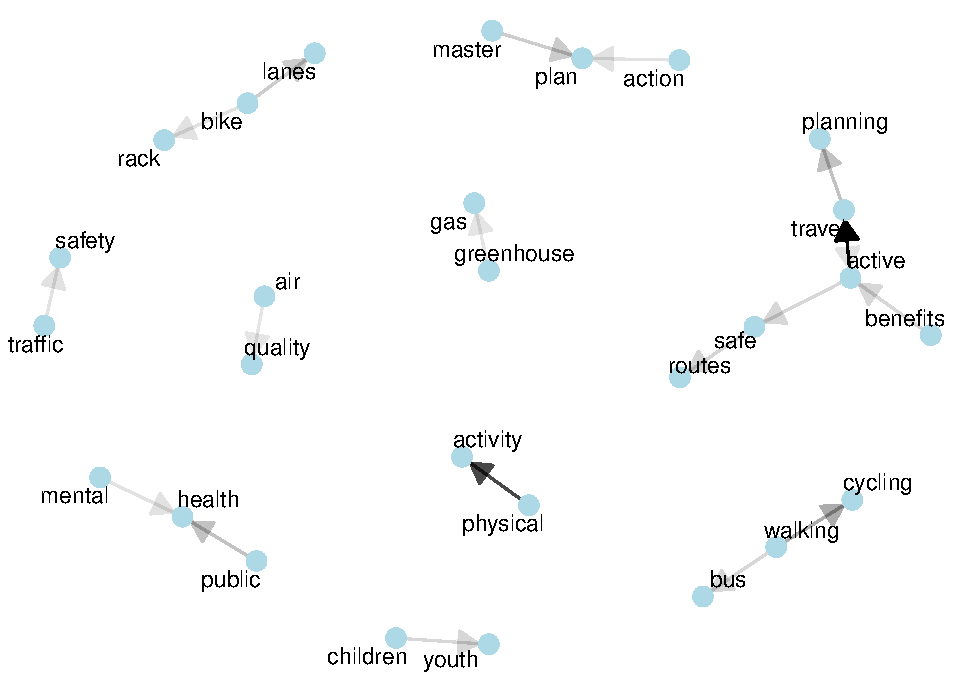
\includegraphics[width=1\linewidth]{AST-Framing-Ontario_files/figure-latex/city-visual-1} 

}

\caption{Most common bigrams found in the municipal or regional government documents.}\label{fig:city-visual}
\end{figure}

\begin{figure}

{\centering 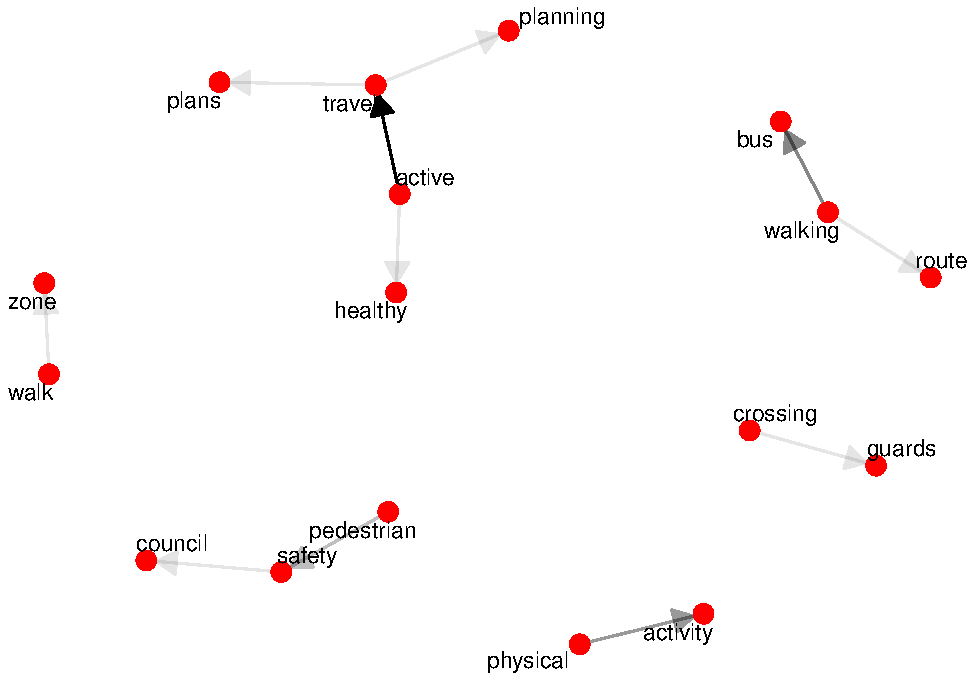
\includegraphics[width=1\linewidth]{AST-Framing-Ontario_files/figure-latex/consortia-visual-1} 

}

\caption{Most common bigrams found in the transportation consortia documents.}\label{fig:consortia-visual}
\end{figure}

\begin{figure}

{\centering 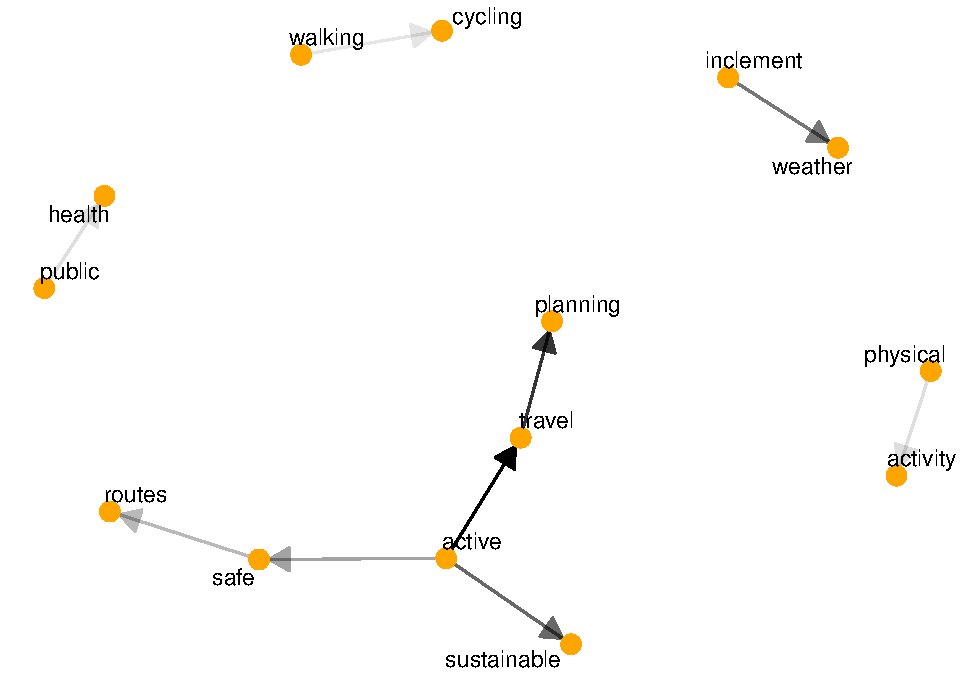
\includegraphics[width=1\linewidth]{AST-Framing-Ontario_files/figure-latex/school-visual-1} 

}

\caption{Most common bigrams found in the school board documents.}\label{fig:school-visual}
\end{figure}

\begin{figure}

{\centering 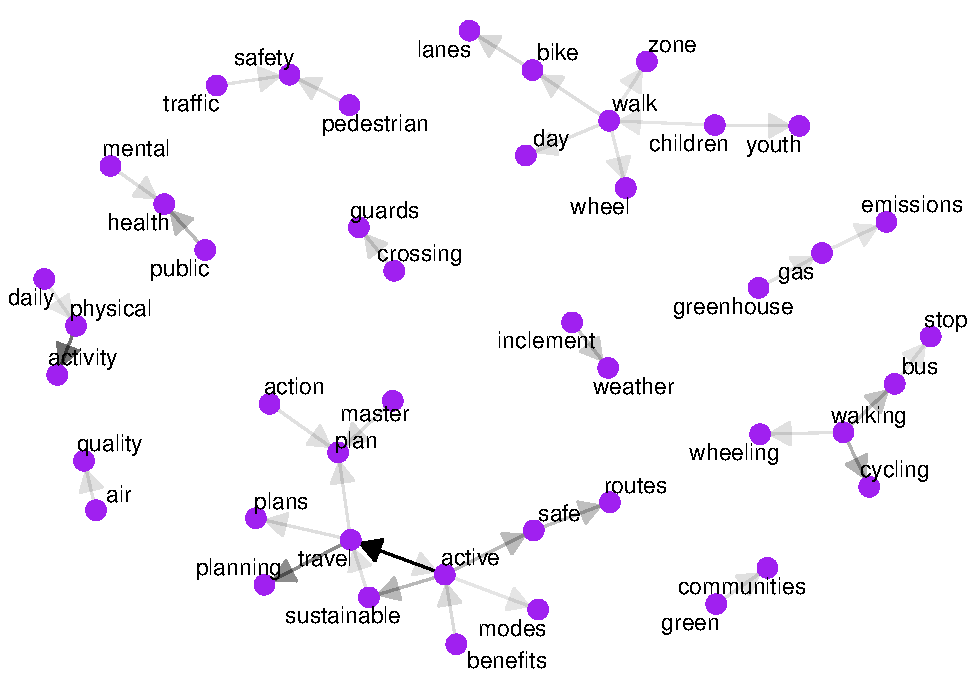
\includegraphics[width=1\linewidth]{AST-Framing-Ontario_files/figure-latex/policy-visual-1} 

}

\caption{Most common bigrams found across all policy documents (i.e., school board, municipality, and transportation consortia combined).}\label{fig:policy-visual}
\end{figure}

We then combined all municipality, school board, and transportation
consortia documents into one ``policy'' corpora. This enabled us to
examine and visualize the most common bigrams found across all of the
STP material in Ontario that was collected for this study. Figure
\ref{fig:policy-visual} shows all of the bigrams that occur more than 10
times in the corpora. In addition to the common bigrams already
identified above, we also found \emph{mental health}, \emph{walk day},
and \emph{green communities} as common pairs of consecutive words.
Overall, policy documents from STP stakeholders seem to focus on four
key areas: i) benefits or impacts of AST; ii) mechanisms of
intervention; iii) concerns or considerations; and iv) supports for AST.

We analyzed bigrams in the academic corpora separately to make
comparisons with the policy corpora. Figure \ref{fig:academic-visual}
indicates that the academic corpora includes several common bigrams that
were also found in the policy documents including \emph{physical
activity} (n = 1566), which is the top bigram, \emph{traffic safety} (n
= 308), and \emph{safe routes} (n = 268). However, many other factors
relating to AST are identified in the research literature that are not
presented to the public through policy documents. After \emph{physical
activity}, \emph{built environment} (n = 1175), \emph{independent
mobility} (n = 774), and \emph{urban form} (n = 352) are the most
frequent pairs of consecutive words. Academic papers also often discuss
\emph{distance home} (n = 258), \emph{car ownership} (n = 254),
\emph{household income} (n = 254), and \emph{population density} (n =
205), which are factors that have been found to influence AST. It is
evident that many papers investigate gender differences in AST given
that \emph{boys girls} (n = 211) is another common bigram. Finally, the
presence of \emph{statistically significant} among the top bigrams
underscores that researchers aim to identify determinants that are not
due to chance but that likely influence AST. The academic corpora
focuses on a greater range of topics than found in the STP material.

\begin{figure}

{\centering 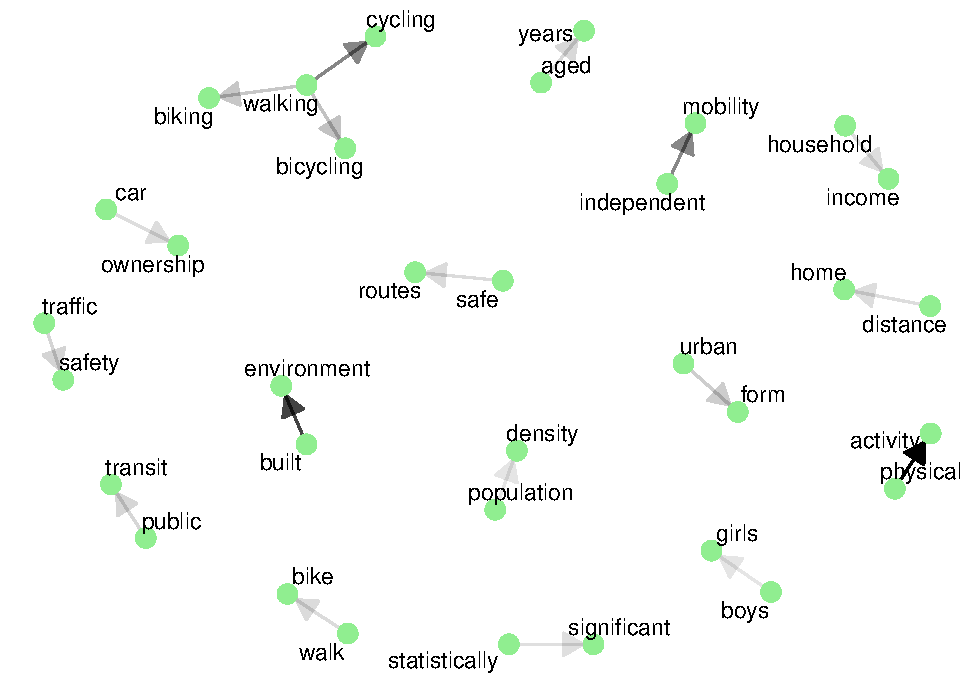
\includegraphics[width=1\linewidth]{AST-Framing-Ontario_files/figure-latex/academic-visual-1} 

}

\caption{Most common bigrams found in the academic papers.}\label{fig:academic-visual}
\end{figure}

We interpreted the most common bigrams from the policy corpora (see
Figure \ref{fig:policy-visual}), which includes all documents from
municipalities, transportation consortia, and school boards, as the main
ideas that STP stakeholders are focusing on and communicating to the
public about AST. We then used the \texttt{kwic} function from the R
\emph{quanteda} package to identify and better understand the context of
these key themes. Table \ref{tab:policy-concordance} presents examples
of the key themes that were extracted from select policy documents to
demonstrate how the most common bigrams are communicated to the public.

\begin{table}
\centering
\begin{tabular}[t]{>{}l|l|>{\raggedright\arraybackslash}p{30em}}
\hline
Terms & Stakeholder & Context\\
\hline
\textbf{Air Quality} & School Board & Active transportation [...] improves air quality.\\
\hline
\textbf{Benefit} & Municipality & Stronger bones and muscles, improved self-esteem and sense of well-being while reducing stress and risk of chronic disease all benefit those who use active transportation.\\
\hline
\textbf{Bus} & School Board & While taking part in a walking school bus, your child will enjoy seeing friends on the way to school. They will be active more often. This is also a great opportunity for your child to socialize with school friends in a monitored and safe way where they can practice social distancing, modelled by a leader.\\
\hline
\textbf{Community} & School Board & Engage community stakeholders (school boards, municipalities, police, public health professionals, parents/guardians, administrators, educators and children) to work together to identify and to solve their school travel needs.\\
\hline
\textbf{Emissions} & Consortia & An active school commute also reduces congestion in school zones and contributes to reducing greenhouse gas emissions – it’s a win-win for everyone!\\
\hline
\textbf{Health} & Municipality & Active School Travel allows school-aged children the chance to participate in moderate to intense physical activity. This is linked with lower body mass index and improved cardiovascular health.\\
\hline
\textbf{Lanes} & Municipality & We are continuing to build on the cycling and pedestrian network by adding more bike lanes, building multi-use paths and encouraging developments to provide better pedestrian/cycling environments.\\
\hline
\textbf{Mental Health} & Municipality & ASST not only improves physical and mental health but contributes to a healthier environment and safer streets.\\
\hline
\textbf{Physical Health} & Municipality & Encouraging Active Transportation promotes personal health and recreation, helps manage congestion, reduces emissions and supports municipal objectives for efficient land use.\\
\hline
\end{tabular}
\end{table}

\hypertarget{topic-modelling-1}{%
\subsection{5.3. Topic modelling}\label{topic-modelling-1}}

\begin{verbatim}
## Warning: `guides(<scale> = FALSE)` is deprecated. Please use `guides(<scale> =
## "none")` instead.
\end{verbatim}

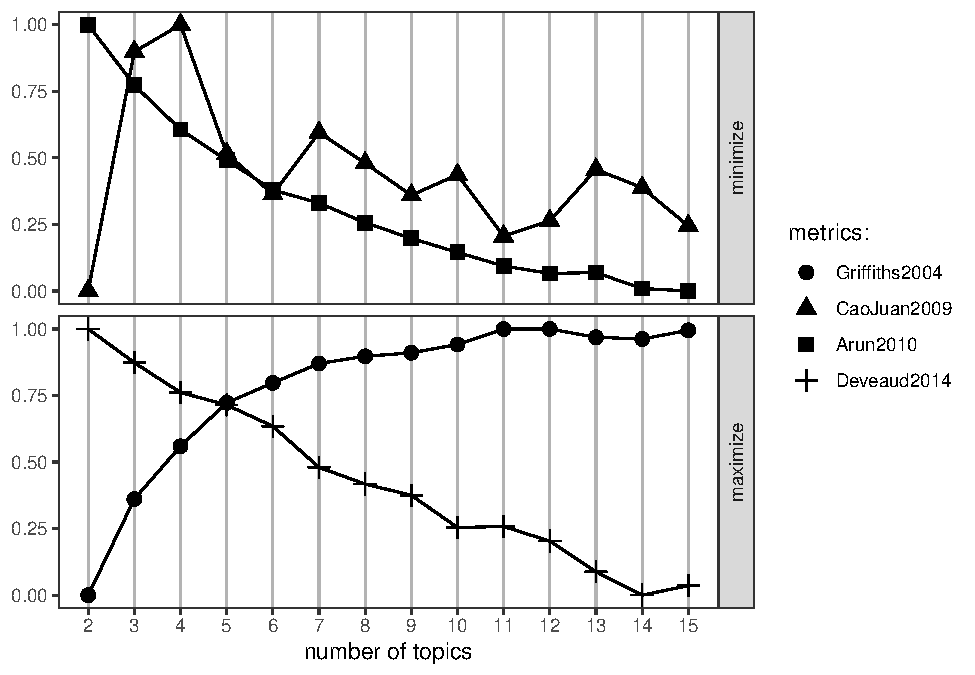
\includegraphics{AST-Framing-Ontario_files/figure-latex/evaluate-lda-1.pdf}

\begin{verbatim}
## Warning: `guides(<scale> = FALSE)` is deprecated. Please use `guides(<scale> =
## "none")` instead.
\end{verbatim}

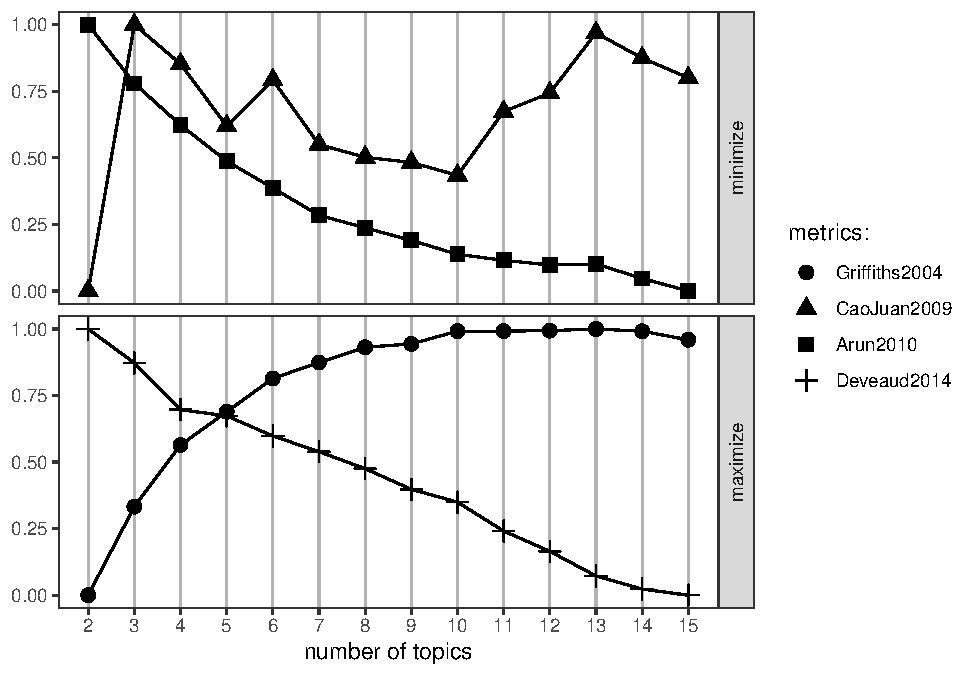
\includegraphics{AST-Framing-Ontario_files/figure-latex/evaluate-lda-2.pdf}

\begin{verbatim}
## Warning: `guides(<scale> = FALSE)` is deprecated. Please use `guides(<scale> =
## "none")` instead.
\end{verbatim}

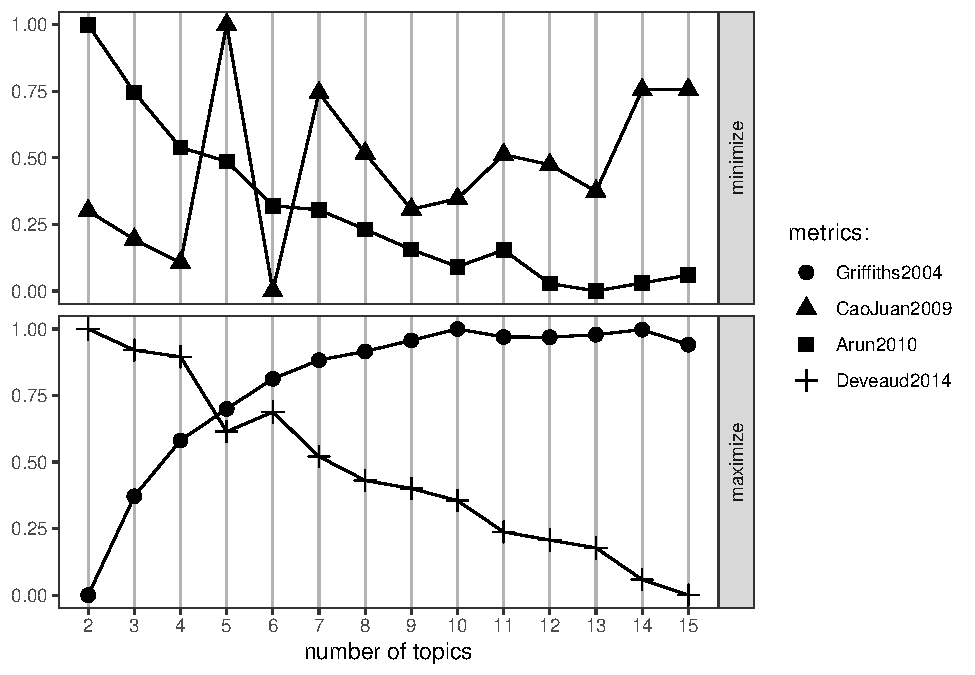
\includegraphics{AST-Framing-Ontario_files/figure-latex/evaluate-lda-3.pdf}

\begin{verbatim}
## Warning: `guides(<scale> = FALSE)` is deprecated. Please use `guides(<scale> =
## "none")` instead.
\end{verbatim}

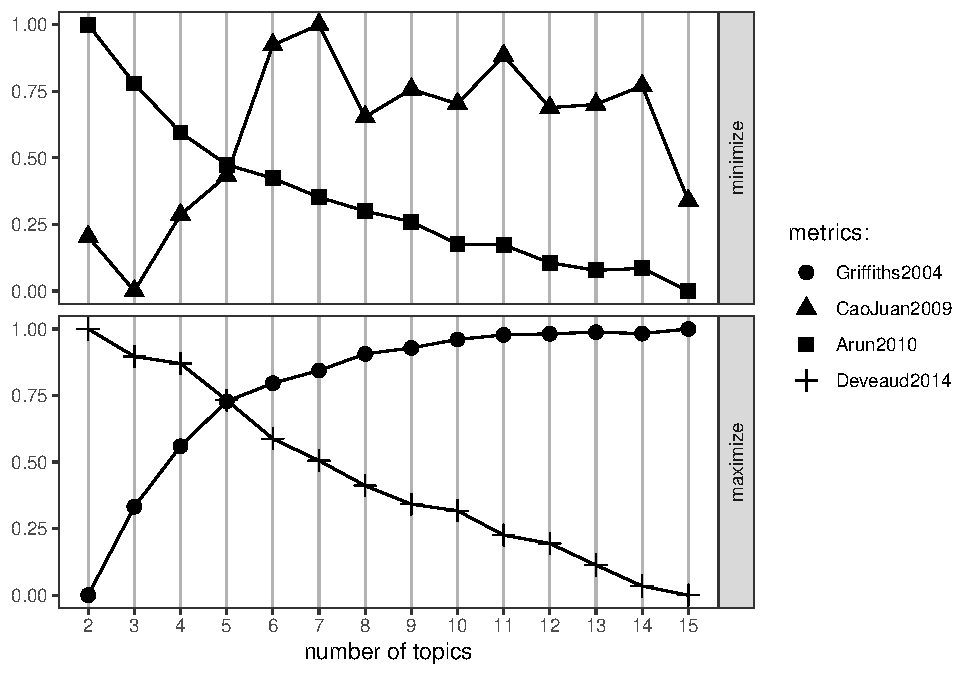
\includegraphics{AST-Framing-Ontario_files/figure-latex/evaluate-lda-4.pdf}

\begin{verbatim}
## Warning: `guides(<scale> = FALSE)` is deprecated. Please use `guides(<scale> =
## "none")` instead.
\end{verbatim}

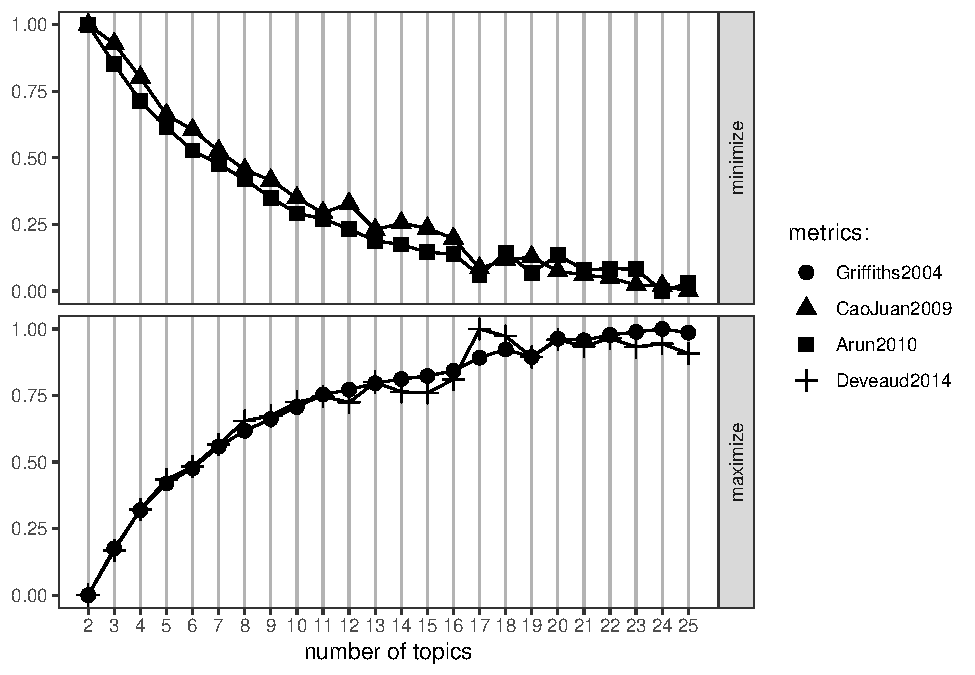
\includegraphics{AST-Framing-Ontario_files/figure-latex/evaluate-lda-5.pdf}

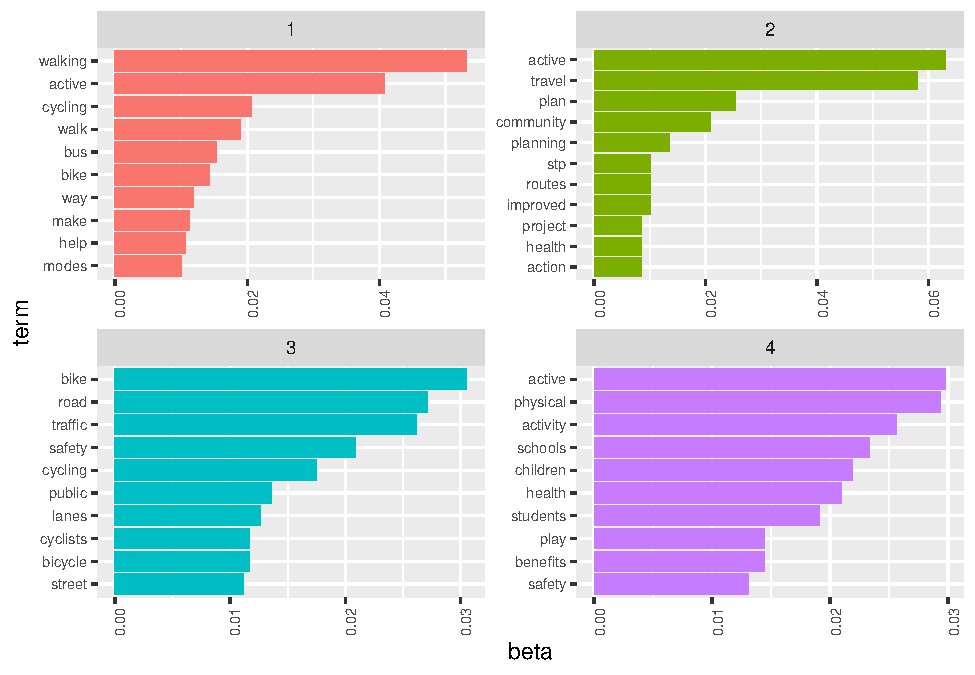
\includegraphics{AST-Framing-Ontario_files/figure-latex/municipal-terms-1.pdf}

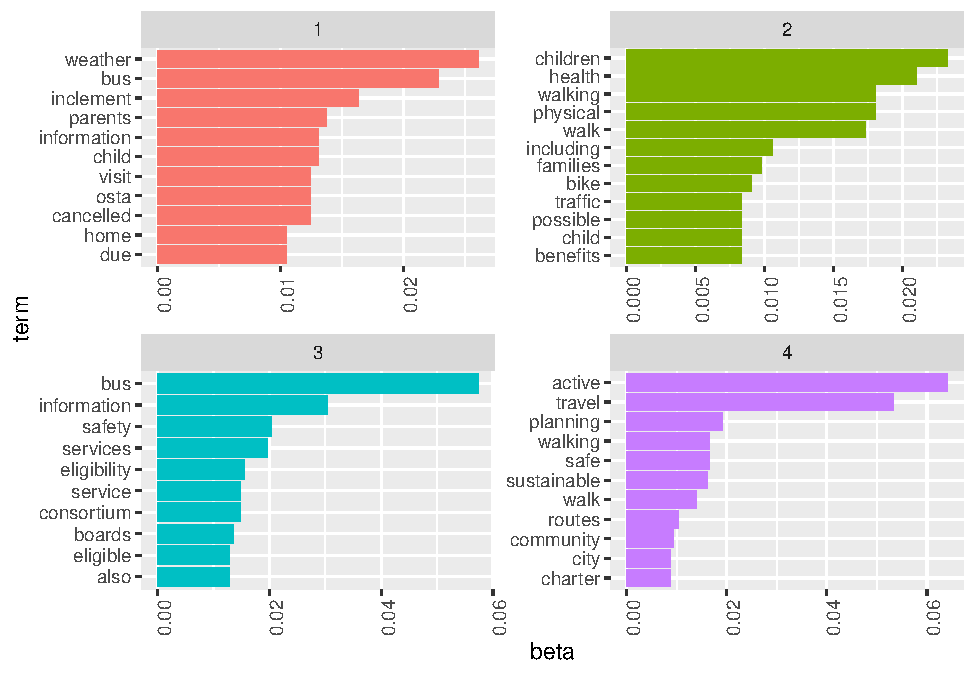
\includegraphics{AST-Framing-Ontario_files/figure-latex/school-terms-1.pdf}

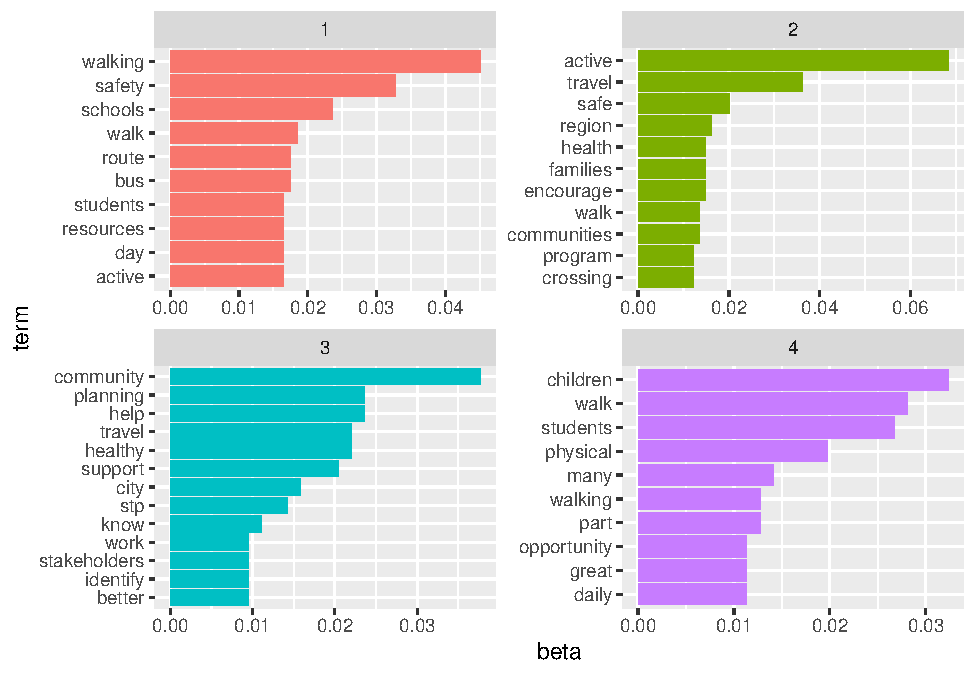
\includegraphics{AST-Framing-Ontario_files/figure-latex/consortia-terms-1.pdf}

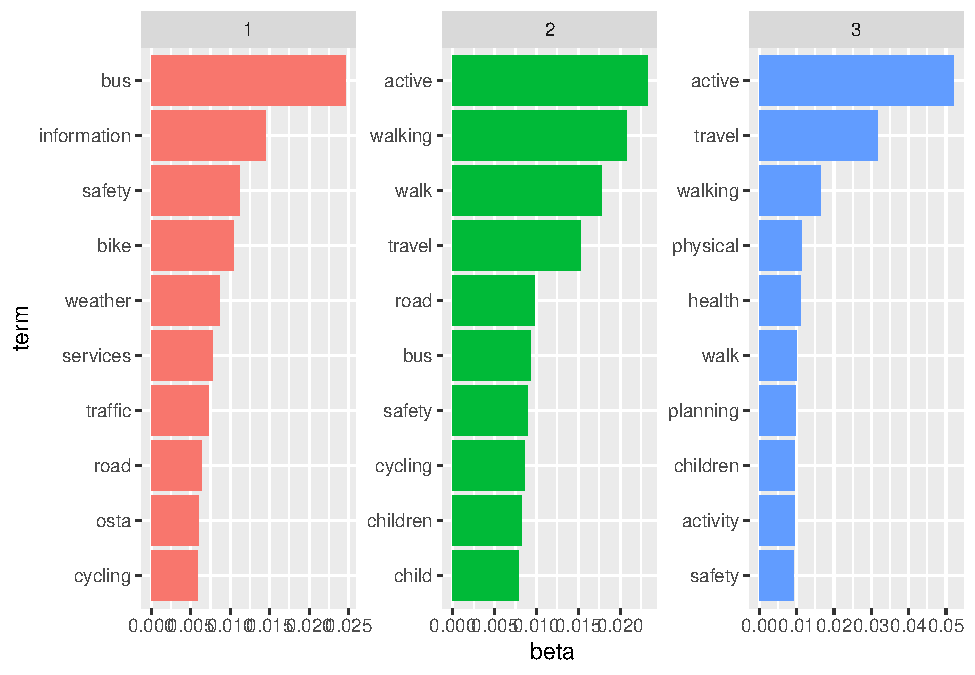
\includegraphics{AST-Framing-Ontario_files/figure-latex/policy-terms-1.pdf}

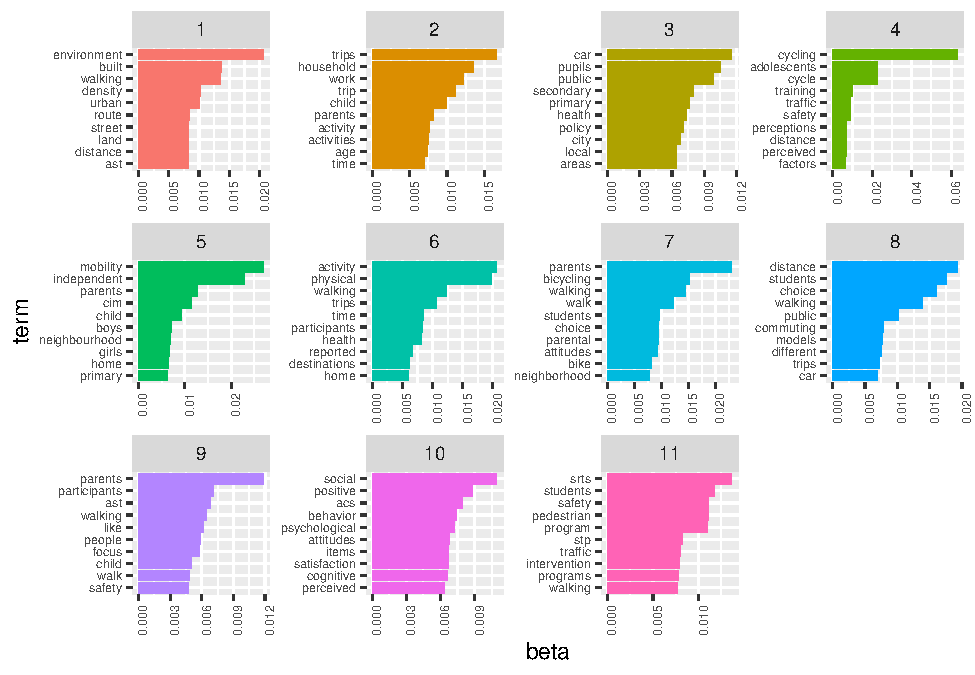
\includegraphics{AST-Framing-Ontario_files/figure-latex/academic-terms-1.pdf}

Finally, we conducted topic modelling to examine the different topics
found in the policy and academic corpora. We focused on the policy
corpora, instead of individually assessing the municipal, school, and
consortia corpus, so that we could report on the primary and secondary
frames used across all documents put out by STP stakeholders in Ontario.
To determine the number of discrete topics in each corpus, we used the
ldatuning package. We then used the \texttt{LDA} function from the
topicmodels package to estimate an LDA model for each group of
documents. The policy corpora, which combined all documents from
municipalities, schools, and transportation consortia, had 5 topics. The
academic corpora had 17 topics. Figures \ref{fig: policy-terms} and
\ref{fig: academic-terms} present the main terms that are associated
with the topics found in each corpus.

In the policy corpus, we identified the following topics: (1) resources
for walking, (2) busing information and eligibility; (3) benefits of
active travel; (4) bicycling and the environment; and (5) supporting
active travel. These findings reveal that STP stakeholders are sending
the message that walking and bicycling to school as healthy travel modes
for students, particularly as a means to get physical activity. We also
found that there is information shared to support parents and students
in using active modes to school such as the availability of cycling
lanes or route tips for walking. STP stakeholders appear to be
communicating that AST is possible and safe as a result of improvements
to the built environment and available resources for parents and
children. A final focus in the policy documents is on various efforts
that are underway to support active travel including route planning.

We expected to find a higher number of topics in the academic corpus due
to the larger number of documents in the corpora and the diversity of
content examined in existing literature about school travel. The
following topics were identified, which touch upon a broader range of
factors that are associated with or related to AST than are found in the
policy corpus: (1) \textbf{unclear} (2) AST in Ontario and Canada; (3)
\textbf{unclear}; (4) children's independent mobility; (5) safe routes
to school programs; (6) commuting and distance; (7) density in the built
environment and walking routes; (8) \textbf{unclear}; (9) walking
interventions; (10) bicycling influences; (11) interpersonal and
household influences on trips; (12) behaviours and attitudes; (13)
\textbf{unclear}; (14) \textbf{unclear}; (15) walking distance; (16)
\textbf{unclear}; (17) physical activity measures or results; (18)
bicycling attitudes; and (19) \textbf{unclear}.

The policy corpus primarily frames AST as a health and environmental
issue. Many municipal and school documents position walking, bicycling,
or rolling to school as beneficial to individual health, including
improvements to physical activity levels or mental health, and to the
broader community through a reduction in traffic and vehicle emissions.
\textgreater{} \emph{If you live in a walk zone, the best way to get to
school is by walking or biking. This promotes physical activity, helps
the environment and minimizes traffic around schools during busy times.}
(City of Barrie)

\begin{quote}
\emph{Walking to school is a great way to add physical activity into
your child's busy day.} (Region of Haldimand-Norfolk Region)
\end{quote}

\begin{quote}
\emph{Active school travel is a great way for children to be physically
active, which is associated with improved physical and mental health,
while making school zones safer, by reducing traffic volumes at and
around schools.}(Region of Leeds, Grenville and Lanark)
\end{quote}

\begin{quote}
\emph{The WCDSB supports active transportation as the preferred method
of transportation to school because it is a healthy choice that has
proven links to greater student achievement.} (Waterloo Catholic
District School Board)
\end{quote}

We found that some of these documents make direct references to topics
found in research on school travel and the built environment. For
example, some policy documents identify programs that have been
researched in the literature and found to be effective, such as walking
school buses, or explain how an increase in AST will reduce parent
safety concerns. \textgreater{} \_ For their health, safety, environment
and community: Kids learn healthy habits and concentrate better in
class; One less car (yours) reduces traffic and parking problems in
school zones; Teach your kids about traffic safety; Start a walking
school bus; your kids make friends in every grade, and that can prevent
bullying.\_ (City of Guelph)

\begin{quote}
\emph{There are lots of benefits in the classroom for children that walk
or cycle to school on a regular basis. Some of these benefits include
improved concentration and better coping with stress. Being outside
helps to prevent feelings of isolation and increases their social
interactions. Walking and biking to school can also save you money and
lead to fewer cars on the road.} (City of Ottawa)
\end{quote}

The secondary frame for AST in municipal documents is the opportunity or
prospect of behaviour change. Some cities and schools explain how
children and parents can leave the car at home and make the journey to
school on foot or by bike by describing efforts to make AST safer. This
frame enables the public to evaluate their own travel decisions and to
access resources (e.g., walking skills checklist) that will help them
make AST a first choice. Some documents communicate what is being done
by the municipalities or schools, like school travel planning, while
others emphasize the active role of the parent in creating opportunities
for AST in their household or neighbourhood. \textgreater{} \emph{School
Travel Planning is a community-based approach that aims to increase the
number of students and adults choosing active and sustainable travel to
get to and from school. This approach addresses concerns about safety,
physical activity, and the environment.} (City of Hamilton)

\begin{quote}
\_A way to make sure your child is safe while walking to school is with
a `walking school bus.' Here are some tips for a walking school bus:
Invite families who live nearby to walk; Pick a route and take a test
walk; Take side streets and paths that are less busy with traffic;
Decide how often the group will walk together; Talk with your boss to
adjust your day; Have fun! (City of Ottawa)
\end{quote}

\begin{quote}
Help your students get started on the right foot -encourage them to walk
or bike to school when possible. Even leaving the car a block or two and
walking the rest of the way helps. It's good for the environment and
your health, and teaches your child independence and community
awareness.\_ (Halton District School Board)
\end{quote}

\begin{quote}
\emph{Today, as more and more of our neighbourhoods are being
retrofitted with new sidewalks and bike lanes, pedestrian crossovers,
street lights, reduced speed limits and/or crossing guards, the walk or
bike ride to and from school has never been easier, safer or healthier.}
(Hamilton-Wentworth District Catholic School Board)
\end{quote}

\begin{quote}
\emph{Want to boost your child's mental and physical health? Ottawa
Public Health, City of Ottawa, and OSTA have produced a tipsheet for
parents about ``active transportation'' to school -- fitting walking and
wheeling into your daily routine.} (Ottawa-Carleton District School
Board)
\end{quote}

Finally, many municipalities, schools, and consortia make no mention of
active school travel on their main website pages for active
transportation. Nonetheless, some municipalities explain how changes to
the built environment are being implemented to facilitate active travel.
Schools or consortia that do not refer to AST simply provide information
about the busing service available to families in the region. Inclement
weather and impacts to busing is a common topic addressed in those
documents. \textgreater{} \emph{We are continuing to build on the
cycling and pedestrian network by adding more bike lanes, building
multi-use paths and encouraging developments to provide better
pedestrian/cycling environments.} (City of Brantford)

\begin{quote}
\emph{The City of Burlington ensures all cyclists, pedestrians and
drivers have access to safe and accessible transportation services and
programs} (City of Burlington)
\end{quote}

\hypertarget{discussion}{%
\section{6. Discussion}\label{discussion}}

\hypertarget{framing-in-stp-documents}{%
\subsection{6.1. Framing in STP
documents}\label{framing-in-stp-documents}}

We analyzed how AST is framed in documents available to the public on
the websites of STP stakeholders in Ontario. We found that AST is
primarily framed as beneficial to the health and wellbeing of children
and to environmental sustainability. This was confirmed by the most
common bigrams identified in the policy corpora, as well as the topics
identified by the LDA model. Many studies and reviews have focused on
the association between AST and physical activity (e.g., Faulkner et
al., 2009; Mitra et al., 2017; Schoeppe et al., 2015), with findings
consistently demonstrating that children who travel by walking or
bicycling to school are more active than their peers who do not use
active travel. More recently, researchers have been exploring the link
between transport and children's wellbeing (Babb et al., 2017), which
has relevant applications to the study of school travel and satisfaction
(see van den Berg et al., 2020). We concluded that STP promotional
materials have high concurrence with this topic in the research on
school travel and the built environment. Framing AST as a health issue
is certainly warranted - there is strong evidence that children who walk
and bicycle to school accrue physical and mental health benefits.
Furthermore, concerns about traffic and strangers have been reported by
parents who drive their children to school (Mammen et al., 2012).
Parents often have concerns about traffic volume, speed, and congestion
around schools (Ling et al., 2021; Rothman et al., 2017), therefore the
framing of AST as an environmental issue is in alignment with evidence
from existing studies.

The secondary frame of AST is that it is a behaviour that can and should
be adopted by children and parents given the environmental and program
supports available in the community. STP stakeholders emphasize that
parents can access resources or trips to support their children in
commuting by active modes to school. They also share information about
interventions such as school travel plans and bicycle lanes to frame AST
as safe and practical. However, STP materials neglect to address many
intrapersonal and household factors that influence or predict AST. At
the individual level, older child age is often associated with AST
({\textbf{???}}; Mammen et al., 2012; Wilson et al., 2018), but AST is
not framed as an activity for children based on age. STP stakeholders
may wish to emphasize to parents that older children have greater
traffic safety and cognitive abilities to navigate their own routes to
school. There is also some evidence that gender is a determinant of AST
({\textbf{???}}; Babb et al., 2017), although this is not a strong or
consistent finding ({\textbf{???}}; Schoeppe et al., 2015). STP
materials do not discuss this determinant of AST but it may be helpful
to identify strategies or messages that alleviate specific concerns that
relate to a child's gender.

Furthermore, distance between home and school is the factor most
associated with AST in existing research ({\textbf{???}}; Ikeda et al.,
2018; Mammen et al., 2012; Pont et al., 2009) with less AST reported
among children who have to travel farther to school. This topic is not
addressed substantively in the policy corpus, perhaps due to the
inability of STP stakeholders to directly intervene in residential
location. Parental perceptions of the environment (De Meester et al.,
2014; Panter et al., 2010) and children's skills (Ghekiere et al., 2017)
also influence whether they allow their children to walk or cycle to
school. STP documents do a sufficiently good job at communicated how an
increase in AST could improve traffic safety in school zones and how new
infrastructure improvements give children the ability to safely travel.
This messaging has high concurrence with studies that have found that
the quality of the built environment (Ikeda et al., 2018; Kim and Lee,
2020) and active travel infrastructure (Pont et al., 2009) facilitate
AST.

To increase rates of walking and bicycling independently to school,
Riazi et al.~(2019) state: ``it will be vital for interventions to
target modifiable factors, including children's and parents' perceptions
of their social environment.'' We argue that STP messaging should also
target multiple modifiable factors, in addition to the health and
environmental benefits. Parents play the important role of
``gatekeeper'' by either granting or restricting their child's mobility
(Sharmin and Kamruzzaman, 2017). For this reason, stakeholders involved
in STP should produce more information that specifically responds to
parents' perceived barriers and challenges. For example, STP materials
could explain how known concerns in a particular municipality or school
area have been addressed through local solutions.

\hypertarget{implications-for-school-travel-planning}{%
\subsection{6.2. Implications for school travel
planning}\label{implications-for-school-travel-planning}}

Many municipalities, schools, and transportation consortia use similar
content in their public documents about AST. It would be worthwhile for
STP stakeholders to adapt generic content so that it is more specific to
factors associated with AST or parental perceptions about barriers to
AST in the local context. Rothman et al.~(2018) note that local
solutions to address specific school challenges are worthwhile, and we
extend this recommendation to include local context in STP messaging
about AST.

\hypertarget{limitations}{%
\subsection{6.3. Limitations}\label{limitations}}

\hypertarget{conclusion}{%
\section{7. Conclusion}\label{conclusion}}

\hypertarget{future-research}{%
\subsection{7.1. Future research}\label{future-research}}

Future studies may investigate how parents and policymakers outside the
field of public health respond to the ways in which AST is framed in STP
documents. It would be helpful to know which frames would most encourage
behaviour change or increase political support for interventions that
address barriers to AST. This type of information could ensure that
educational strategies and promotional materials increase buy-in for
their target audience.

\hypertarget{acknowledgments}{%
\section{Acknowledgments}\label{acknowledgments}}

This research was completed using open software, and the authors wish to
acknowledge the developers of the following \texttt{R} packages:
\texttt{dplyr} ({\textbf{???}}), \texttt{ggraph} ({\textbf{???}}),
\texttt{ggplot2} ({\textbf{???}}), \texttt{igraph} ({\textbf{???}}),
\texttt{pdftools} ({\textbf{???}}), \texttt{readr} ({\textbf{???}}),
\texttt{reshape2} ({\textbf{???}}), \texttt{stringr} ({\textbf{???}}),
\texttt{text2vec} ({\textbf{???}}), \texttt{textdata} ({\textbf{???}}),
\texttt{tidyr} ({\textbf{???}}), \texttt{tidytext} ({\textbf{???}}),
\texttt{tm} ({\textbf{???}}), \texttt{tools} ({\textbf{???}}),
\texttt{topicmodels} ({\textbf{???}}), \texttt{widyr} ({\textbf{???}}),
\texttt{word2vec} ({\textbf{???}}), \texttt{wordcloud} ({\textbf{???}}),
\texttt{DiagrammeR} ({\textbf{???}}), and \texttt{kableextra}
({\textbf{???}}).

\hypertarget{references}{%
\section*{References}\label{references}}
\addcontentsline{toc}{section}{References}

\hypertarget{refs}{}
\leavevmode\hypertarget{ref-babbChildrenActiveTravel2017}{}%
Babb, C., Olaru, D., Curtis, C., Robertson, D., 2017. Children's active
travel, local activity spaces and wellbeing: A case study in Perth, WA.
Travel Behaviour and Society 9, 81--94.
doi:\href{https://doi.org/10.1016/j.tbs.2017.06.002}{10.1016/j.tbs.2017.06.002}

\leavevmode\hypertarget{ref-buliungLivingJourneySchool2021}{}%
Buliung, R., Hess, P., Flowers, L., Moola, F.J., Faulkner, G., 2021.
Living the journey to school: Conceptual asymmetry between parents and
planners on the journey to school. Social Science \& Medicine 284,
114237.
doi:\href{https://doi.org/10.1016/j.socscimed.2021.114237}{10.1016/j.socscimed.2021.114237}

\leavevmode\hypertarget{ref-buttazzoniPromotingActiveSchool2019}{}%
Buttazzoni, A.N., Clark, A.F., Seabrook, J.A., Gilliland, J.A., 2019.
Promoting active school travel in elementary schools: A regional case
study of the school travel planning intervention. Journal of Transport
\& Health 12, 206--219.
doi:\href{https://doi.org/10.1016/j.jth.2019.01.007}{10.1016/j.jth.2019.01.007}

\leavevmode\hypertarget{ref-demeesterParentalPerceivedNeighborhood2014}{}%
De Meester, F., Van Dyck, D., De Bourdeaudhuij, I., Cardon, G., 2014.
Parental perceived neighborhood attributes: Associations with active
transport and physical activity among 10-12 year old children and the
mediating role of independent mobility. BMC public health 14, 631.
doi:\href{https://doi.org/10.1186/1471-2458-14-631}{10.1186/1471-2458-14-631}

\leavevmode\hypertarget{ref-faulknerActiveSchoolTransport2009}{}%
Faulkner, G.E.J., Buliung, R.N., Flora, P.K., Fusco, C., 2009. Active
school transport, physical activity levels and body weight of children
and youth: A systematic review. Preventive Medicine 48, 3--8.
doi:\href{https://doi.org/10.1016/j.ypmed.2008.10.017}{10.1016/j.ypmed.2008.10.017}

\leavevmode\hypertarget{ref-ghekiereInsightsChildrenIndependent2017}{}%
Ghekiere, A., Deforche, B., Carver, A., Mertens, L., de Geus, B.,
Clarys, P., Cardon, G., De Bourdeaudhuij, I., Van Cauwenberg, J., 2017.
Insights into children's independent mobility for transportation
cyclingWhich socio-ecological factors matter? Journal of Science and
Medicine in Sport 20, 267--272.
doi:\href{https://doi.org/10.1016/j.jsams.2016.08.002}{10.1016/j.jsams.2016.08.002}

\leavevmode\hypertarget{ref-goffmanFrameAnalysisEssay1974}{}%
Goffman, E., 1974. Frame analysis: An essay on the organization of
experience, Frame analysis: An essay on the organization of experience.
Harvard University Press, Cambridge, MA, US.

\leavevmode\hypertarget{ref-ikedaAssociationsChildrenActive2018}{}%
Ikeda, E., Hinckson, E., Witten, K., Smith, M., 2018. Associations of
children's active school travel with perceptions of the physical
environment and characteristics of the social environment: A systematic
review. Health \& Place 54, 118--131.
doi:\href{https://doi.org/10.1016/j.healthplace.2018.09.009}{10.1016/j.healthplace.2018.09.009}

\leavevmode\hypertarget{ref-kimBuiltNaturalEnvironmental2020}{}%
Kim, Y.-J., Lee, C., 2020. Built and Natural Environmental Correlates of
Parental Safety Concerns for Children's Active Travel to School.
International Journal of Environmental Research and Public Health 17.
doi:\href{https://doi.org/10.3390/ijerph17020517}{10.3390/ijerph17020517}

\leavevmode\hypertarget{ref-lingRelationshipMotorVehicle2021}{}%
Ling, R., Rothman, L., Hagel, B., Macarthur, C., Winters, M., Churchill,
T., HubkaRao, T., Macpherson, A., Cloutier, M.-S., Howard, A., 2021. The
relationship between motor vehicle speed and active school
transportation at elementary schools in Calgary and Toronto, Canada.
Journal of Transport \& Health 21, 101034.
doi:\href{https://doi.org/10.1016/j.jth.2021.101034}{10.1016/j.jth.2021.101034}

\leavevmode\hypertarget{ref-mahFramecriticalPolicyAnalysis2014}{}%
Mah, C.L., Hamill, C., Rondeau, K., McIntyre, L., 2014. A frame-critical
policy analysis of Canada's response to the World Food Summit 19982008.
Archives of Public Health 72, 41.
doi:\href{https://doi.org/10.1186/2049-3258-72-41}{10.1186/2049-3258-72-41}

\leavevmode\hypertarget{ref-maibachReframingClimateChange2010}{}%
Maibach, E.W., Nisbet, M., Baldwin, P., Akerlof, K., Diao, G., 2010.
Reframing climate change as a public health issue: An exploratory study
of public reactions. BMC Public Health 10, 1--11.
doi:\href{https://doi.org/10.1186/1471-2458-10-299}{10.1186/1471-2458-10-299}

\leavevmode\hypertarget{ref-mammenUnderstandingDriveEscort2012}{}%
Mammen, G., Faulkner, G., Buliung, R., Lay, J., 2012. Understanding the
drive to escort: A cross-sectional analysis examining parental attitudes
towards children's school travel and independent mobility. BMC public
health 12, 862.
doi:\href{https://doi.org/10.1186/1471-2458-12-862}{10.1186/1471-2458-12-862}

\leavevmode\hypertarget{ref-mammenActiveSchoolTravel2014}{}%
Mammen, G., Stone, M.R., Faulkner, G., Ramanathan, S., Buliung, R.,
O'Brien, C., Kennedy, J., 2014. Active school travel: An evaluation of
the Canadian school travel planning intervention. Preventive Medicine
60, 55--59.
doi:\href{https://doi.org/10.1016/j.ypmed.2013.12.008}{10.1016/j.ypmed.2013.12.008}

\leavevmode\hypertarget{ref-mitraChildrenActivitytransportationLifestyles2017}{}%
Mitra, R., Cantello, I.D., Buliung, R.N., Faulkner, G.E.J., 2017.
Children's activity-transportation lifestyles, physical activity levels
and social-ecological correlates in Toronto, Canada. Journal of
Transport \& Health 6, 289--298.
doi:\href{https://doi.org/10.1016/j.jth.2017.03.010}{10.1016/j.jth.2017.03.010}

\leavevmode\hypertarget{ref-panFramingAnalysisApproach1993}{}%
Pan, Z., Kosicki, G.M., 1993. Framing analysis: An approach to news
discourse. Political Communication 10, 55--75.
doi:\href{https://doi.org/10.1080/10584609.1993.9962963}{10.1080/10584609.1993.9962963}

\leavevmode\hypertarget{ref-panterAttitudesSocialSupport2010}{}%
Panter, J.R., Jones, A.P., Sluijs, E.M.F. van, Griffin, S.J., 2010.
Attitudes, social support and environmental perceptions as predictors of
active commuting behaviour in school children. Journal of Epidemiology
\& Community Health 64, 41--48.
doi:\href{https://doi.org/10.1136/jech.2009.086918}{10.1136/jech.2009.086918}

\leavevmode\hypertarget{ref-pontEnvironmentalCorrelatesChildren2009}{}%
Pont, K., Ziviani, J., Wadley, D., Bennett, S., Abbott, R., 2009.
Environmental correlates of children's active transportation: A
systematic literature review. Health \& Place 15, 849--862.
doi:\href{https://doi.org/10.1016/j.healthplace.2009.02.002}{10.1016/j.healthplace.2009.02.002}

\leavevmode\hypertarget{ref-riaziCorrelatesChildrenIndependent2019}{}%
Riazi, N.A., Blanchette, S., Trudeau, F., Larouche, R., Tremblay, M.S.,
Faulkner, G., 2019. Correlates of Children's Independent Mobility in
Canada: A Multi-Site Study. International Journal of Environmental
Research and Public Health 16.
doi:\href{https://doi.org/10.3390/ijerph16162862}{10.3390/ijerph16162862}

\leavevmode\hypertarget{ref-rothmanSchoolEnvironmentStudent2017}{}%
Rothman, L., Buliung, R., Howard, A., Macarthur, C., Macpherson, A.,
2017. The school environment and student car drop-off at elementary
schools. Travel Behaviour and Society 9, 50--57.
doi:\href{https://doi.org/10.1016/j.tbs.2017.03.001}{10.1016/j.tbs.2017.03.001}

\leavevmode\hypertarget{ref-rothmanDeclineActiveSchool2018a}{}%
Rothman, L., Macpherson, A.K., Ross, T., Buliung, R.N., 2018. The
decline in active school transportation (AST): A systematic review of
the factors related to AST and changes in school transport over time in
North America. Preventive Medicine 111, 314--322.
doi:\href{https://doi.org/10.1016/j.ypmed.2017.11.018}{10.1016/j.ypmed.2017.11.018}

\leavevmode\hypertarget{ref-schoeppeAssociationsChildrenActive2015}{}%
Schoeppe, S., Duncan, M.J., Badland, H.M., Oliver, M., Browne, M., 2015.
Associations between children׳s active travel and levels of physical
activity and sedentary behavior. Journal of Transport \& Health 2,
336--342.
doi:\href{https://doi.org/10.1016/j.jth.2015.05.001}{10.1016/j.jth.2015.05.001}

\leavevmode\hypertarget{ref-sharminAssociationBuiltEnvironment2017}{}%
Sharmin, S., Kamruzzaman, M., 2017. Association between the built
environment and children's independent mobility: A meta-analytic review.
Journal of Transport Geography 61, 104--117.
doi:\href{https://doi.org/10.1016/j.jtrangeo.2017.04.004}{10.1016/j.jtrangeo.2017.04.004}

\leavevmode\hypertarget{ref-vandenbergFactorsAffectingParental2020}{}%
van den Berg, P., Waygood, E.O.D., van de Craats, I., Kemperman, A.,
2020. Factors affecting parental safety perception, satisfaction with
school travel and mood in primary school children in the Netherlands.
Journal of Transport \& Health 16, 100837.
doi:\href{https://doi.org/10.1016/j.jth.2020.100837}{10.1016/j.jth.2020.100837}

\leavevmode\hypertarget{ref-weathersDevelopmentsFramingClimate2016}{}%
Weathers, M.R., Kendall, B.E., 2016. Developments in the Framing of
Climate Change as a Public Health Issue in US Newspapers. Environmental
Communication 10, 593--611.
doi:\href{https://doi.org/10.1080/17524032.2015.1050436}{10.1080/17524032.2015.1050436}

\leavevmode\hypertarget{ref-wilsonUnderstandingChildParent2018}{}%
Wilson, K., Clark, A.F., Gilliland, J.A., 2018. Understanding child and
parent perceptions of barriers influencing children's active school
travel. BMC public health 18, 1053.
doi:\href{https://doi.org/10.1186/s12889-018-5874-y}{10.1186/s12889-018-5874-y}


\end{document}

